% ══════════════════════════════════════════════════════════════════════════════
%  AUTOMOTIVE QA INTELLIGENCE — SYSTEM ARCHITECTURE & TECHNICAL DOCUMENTATION
%  Enterprise-Grade LaTeX Document
%  Version 1.1 | Confidential — Internal Engineering Use Only
% ══════════════════════════════════════════════════════════════════════════════

\documentclass[12pt, a4paper, twoside]{article}

% ── Packages ──────────────────────────────────────────────────────────────────
\usepackage[utf8]{inputenc}
\usepackage[T1]{fontenc}
\usepackage{lmodern}
\usepackage[margin=1in, headheight=15pt]{geometry}
\usepackage{graphicx}
\usepackage{xcolor}
\usepackage{tikz}
\usetikzlibrary{
  shapes.geometric, arrows.meta, positioning, fit, calc,
  backgrounds, shadows.blur, decorations.markings, patterns,
  matrix, chains
}
\usepackage{pgfplots}
\pgfplotsset{compat=1.18}
\usepackage{booktabs}
\usepackage{longtable}
\usepackage{tabularx}
\usepackage{array}
\usepackage{multirow}
\usepackage{colortbl}
\usepackage{enumitem}
\usepackage{fancyhdr}
\usepackage{titlesec}
\usepackage{tcolorbox}
\tcbuselibrary{skins, breakable}
\usepackage{hyperref}
\usepackage{listings}
\usepackage{float}
\usepackage{caption}
\usepackage{subcaption}
\usepackage{amsmath}
\usepackage{fontawesome5}
\usepackage{pifont}
\usepackage{etoolbox}
\usepackage{setspace}
\usepackage{parskip}
\usepackage{microtype}

% ── Color Palette ─────────────────────────────────────────────────────────────
\definecolor{navy}{HTML}{0F172A}
\definecolor{darknavy}{HTML}{1E3A8A}
\definecolor{skyblue}{HTML}{0EA5E9}
\definecolor{teal}{HTML}{0D9488}
\definecolor{emerald}{HTML}{10B981}
\definecolor{amber}{HTML}{F59E0B}
\definecolor{rose}{HTML}{F43F5E}
\definecolor{slate50}{HTML}{F8FAFC}
\definecolor{slate100}{HTML}{F1F5F9}
\definecolor{slate200}{HTML}{E2E8F0}
\definecolor{slate300}{HTML}{CBD5E1}
\definecolor{slate400}{HTML}{94A3B8}
\definecolor{slate500}{HTML}{64748B}
\definecolor{slate600}{HTML}{475569}
\definecolor{slate700}{HTML}{334155}
\definecolor{slate800}{HTML}{1E293B}
\definecolor{indigo}{HTML}{4F46E5}
\definecolor{violet}{HTML}{7C3AED}
\definecolor{lightblue}{HTML}{EFF6FF}
\definecolor{lightteal}{HTML}{F0FDFA}
\definecolor{lightamber}{HTML}{FFFBEB}
\definecolor{lightrose}{HTML}{FFF1F2}
\definecolor{codebg}{HTML}{0F172A}
\definecolor{codetext}{HTML}{E2E8F0}

% ── Hyperref Setup ────────────────────────────────────────────────────────────
\hypersetup{
  colorlinks=true,
  linkcolor=darknavy,
  urlcolor=skyblue,
  citecolor=teal,
  pdftitle={Automotive QA Intelligence — System Architecture Documentation},
  pdfauthor={Senior Solutions Architect},
  pdfsubject={Technical Architecture Documentation},
}

% ── Header & Footer ──────────────────────────────────────────────────────────
\pagestyle{fancy}
\fancyhf{}
\fancyhead[L]{\small\color{slate500}\textbf{AUTOMOTIVE QA INTELLIGENCE}}
\fancyhead[R]{\small\color{slate500}System Architecture Documentation v1.1}
\fancyfoot[C]{\small\color{slate400}Page \thepage}
\fancyfoot[L]{\scriptsize\color{slate400}CONFIDENTIAL — INTERNAL USE ONLY}
\fancyfoot[R]{\scriptsize\color{slate400}\today}
\renewcommand{\headrulewidth}{0.4pt}
\renewcommand{\footrulewidth}{0.2pt}
\renewcommand{\headrule}{\color{skyblue}\hrule width\headwidth height\headrulewidth}

% ── Section Styling ───────────────────────────────────────────────────────────
\titleformat{\section}
  {\LARGE\bfseries\color{navy}}
  {\thesection.}{0.5em}{}
  [\vspace{-0.5em}{\color{skyblue}\rule{\linewidth}{2pt}}]

\titleformat{\subsection}
  {\large\bfseries\color{darknavy}}
  {\thesubsection}{0.5em}{}

\titleformat{\subsubsection}
  {\normalsize\bfseries\color{slate700}}
  {\thesubsubsection}{0.5em}{}

% ── Code Listing Style ───────────────────────────────────────────────────────
\lstdefinestyle{codestyle}{
  backgroundcolor=\color{codebg},
  basicstyle=\ttfamily\small\color{codetext},
  keywordstyle=\color{skyblue}\bfseries,
  stringstyle=\color{emerald},
  commentstyle=\color{slate400}\itshape,
  breaklines=true,
  frame=single,
  rulecolor=\color{slate700},
  xleftmargin=8pt,
  xrightmargin=8pt,
  framexleftmargin=5pt,
  tabsize=2,
  showstringspaces=false,
}
\lstset{style=codestyle}

% ── Custom tcolorbox Environments ─────────────────────────────────────────────
\newtcolorbox{infobox}[1][]{
  colback=lightblue,
  colframe=skyblue,
  coltitle=white,
  fonttitle=\bfseries,
  title={#1},
  arc=3pt,
  boxrule=1pt,
  left=8pt, right=8pt, top=6pt, bottom=6pt,
  breakable
}

\newtcolorbox{warnbox}[1][]{
  colback=lightamber,
  colframe=amber,
  coltitle=white,
  fonttitle=\bfseries,
  title={#1},
  arc=3pt,
  boxrule=1pt,
  left=8pt, right=8pt, top=6pt, bottom=6pt,
  breakable
}

\newtcolorbox{keybox}[1][]{
  colback=lightteal,
  colframe=teal,
  coltitle=white,
  fonttitle=\bfseries,
  title={#1},
  arc=3pt,
  boxrule=1pt,
  left=8pt, right=8pt, top=6pt, bottom=6pt,
  breakable
}

\newtcolorbox{dangerbox}[1][]{
  colback=lightrose,
  colframe=rose,
  coltitle=white,
  fonttitle=\bfseries,
  title={#1},
  arc=3pt,
  boxrule=1pt,
  left=8pt, right=8pt, top=6pt, bottom=6pt,
  breakable
}

% ── Custom Table Column Types ─────────────────────────────────────────────────
\newcolumntype{L}[1]{>{\raggedright\arraybackslash}p{#1}}
\newcolumntype{C}[1]{>{\centering\arraybackslash}p{#1}}
\newcolumntype{R}[1]{>{\raggedleft\arraybackslash}p{#1}}

% ── TikZ Styles ──────────────────────────────────────────────────────────────
\tikzset{
  % Component blocks
  component/.style={
    rectangle, rounded corners=4pt, minimum width=2.8cm, minimum height=1cm,
    draw=#1!80, fill=#1!10, text=navy, font=\small\bfseries,
    align=center, text width=2.6cm
  },
  component/.default=skyblue,
  % Layer boxes
  layer/.style={
    rectangle, rounded corners=6pt, draw=#1!60, fill=#1!5,
    inner sep=10pt, font=\small\bfseries, text=#1!80
  },
  layer/.default=slate400,
  % Arrow styles
  flow/.style={-{Stealth[length=3mm]}, thick, color=slate600},
  dataflow/.style={-{Stealth[length=3mm]}, thick, color=skyblue, dashed},
  bidirectional/.style={{Stealth[length=3mm]}-{Stealth[length=3mm]}, thick, color=teal},
  % Labels
  flowlabel/.style={font=\scriptsize\itshape, color=slate500, fill=white, inner sep=2pt},
  layerlabel/.style={font=\footnotesize\bfseries, color=#1!80},
  layerlabel/.default=slate600,
}

% ══════════════════════════════════════════════════════════════════════════════
%  DOCUMENT BEGINS
% ══════════════════════════════════════════════════════════════════════════════
\begin{document}

% ── COVER PAGE ────────────────────────────────────────────────────────────────
\thispagestyle{empty}
\begin{tikzpicture}[remember picture, overlay]
  % Navy top band
  \fill[navy] (current page.north west) rectangle ([yshift=-4cm]current page.north east);
  % Sky-blue accent strip
  \fill[skyblue] ([yshift=-4cm]current page.north west) rectangle ([yshift=-4.3cm]current page.north east);
  % Bottom band
  \fill[slate100] (current page.south west) rectangle ([yshift=2cm]current page.south east);
  \fill[navy] ([yshift=2cm]current page.south west) rectangle ([yshift=2.15cm]current page.south east);
\end{tikzpicture}

\vspace*{1.5cm}

\begin{center}
  {\color{white}\Huge\bfseries Automotive QA Intelligence}\\[0.4cm]
  {\color{slate300}\Large System Architecture \& Technical Documentation}
\end{center}

\vspace{3cm}

\begin{center}
  {\color{skyblue}\rule{6cm}{1.5pt}}\\[1cm]
  {\color{slate600}\large Comprehensive Technical Reference}\\[0.3cm]
  {\color{slate500}\normalsize Offline RAG-Powered Automotive Quality Analytics \& Diagnostics Platform}\\[2cm]

  \begin{tabular}{rl}
    \color{slate500}\textbf{Document Version:} & \color{slate700} 1.1 \\[4pt]
    \color{slate500}\textbf{Date:} & \color{slate700} \today \\[4pt]
    \color{slate500}\textbf{Classification:} & \color{rose}\textbf{CONFIDENTIAL — INTERNAL} \\[4pt]
    \color{slate500}\textbf{Prepared by:} & \color{slate700} Senior Solutions Architect \\[4pt]
    \color{slate500}\textbf{Technology Stack:} & \color{slate700} Python · Streamlit · FAISS · Phi-3 · SQLite \\
  \end{tabular}
\end{center}

\vfill
\begin{center}
  {\color{slate400}\footnotesize This document contains proprietary and confidential information.\\
  Unauthorized distribution is strictly prohibited.}
\end{center}

\newpage

% ── TABLE OF CONTENTS ─────────────────────────────────────────────────────────
\thispagestyle{fancy}
\tableofcontents
\newpage

% ══════════════════════════════════════════════════════════════════════════════
%  SECTION 1: SYSTEM OVERVIEW
% ══════════════════════════════════════════════════════════════════════════════
\section{System Overview}

\textbf{Automotive QA Intelligence} is a fully offline, enterprise-grade quality analytics and diagnostics platform designed for automotive Field Technical Information Report (FTIR) analysis. The system enables technicians and quality engineers to perform natural language queries against a structured database of historical vehicle failure records, leveraging a hybrid Retrieval-Augmented Generation (RAG) architecture.

\subsection{Core Objectives}

\begin{itemize}[leftmargin=*, itemsep=4pt]
  \item \textbf{Offline-First Architecture:} Operates entirely without internet connectivity using local LLM inference (Phi-3 Mini 4K via \texttt{llama.cpp}) and local FAISS vector indexing.
  \item \textbf{Hybrid Retrieval:} Combines SQL keyword search, FAISS cosine similarity vector search, and NLP entity extraction for precise multi-strategy information retrieval.
  \item \textbf{Intelligent Query Routing:} An NLP pipeline classifies user intent (\texttt{SEARCH}, \texttt{ANALYTICS}, \texttt{VISUALIZE}, \texttt{COMPARE}, \texttt{REPORT}) and dispatches queries to the optimal processing backend.
  \item \textbf{Dynamic Analytics:} LLM-generated SQL queries enable ad-hoc analytics without pre-defined report templates.
  \item \textbf{Automated Report Generation:} Monthly PDF and DOCX quality reports are compiled dynamically from database aggregations.
  \item \textbf{Enterprise UI:} A Streamlit-based web interface with multi-session chat, real-time data visualization (Plotly), and citation-backed responses.
\end{itemize}

\begin{keybox}[\faIcon{star} Key Differentiator]
Unlike cloud-based AI platforms, this system operates \textbf{entirely offline} with no API keys, no external network calls, and no data egress — making it suitable for air-gapped automotive manufacturing environments where data confidentiality is paramount.
\end{keybox}

\subsection{System Specifications}

\begin{table}[H]
\centering
\caption{Core System Specifications}
\label{tab:specs}
\rowcolors{2}{slate50}{white}
\begin{tabularx}{\textwidth}{>{\bfseries\color{darknavy}}l X}
\toprule
\rowcolor{navy}\color{white}\textbf{Parameter} & \color{white}\textbf{Specification} \\
\midrule
LLM Engine         & Microsoft Phi-3 Mini 4K Instruct (Q4 GGUF, 3.8B parameters) \\
Embedding Model    & all-MiniLM-L6-v2 (SentenceTransformers, 384-dimensional) \\
Vector Index       & FAISS IndexFlatIP with IDMap (Cosine Similarity) \\
Database           & SQLite 3 with WAL mode + 5 Materialized Views \\
Frontend           & Streamlit 1.x with custom enterprise CSS theme \\
Visualization      & Plotly Express + Plotly Graph Objects (6 chart types) \\
LLM Runtime        & llama-cpp-python with NVIDIA CUDA GPU offloading \\
Report Formats     & PDF (ReportLab) + DOCX (python-docx) \\
Deployment         & Single-node local / on-premise (Windows/Linux) \\
\bottomrule
\end{tabularx}
\end{table}

\newpage

% ══════════════════════════════════════════════════════════════════════════════
%  SECTION 2: END-TO-END ARCHITECTURE
% ══════════════════════════════════════════════════════════════════════════════
\section{End-to-End Architecture}

The system follows a \textbf{layered architecture} pattern with clear separation of concerns across six layers: Presentation, Application Logic, Intelligence (AI/ML), Data Access, Storage, and Infrastructure.

\subsection{Layered Architecture Diagram}

\begin{figure}[H]
\centering
\begin{tikzpicture}[node distance=0.3cm, every node/.style={font=\small}]

  % ── Layer 1: Presentation ──
  \node[component=skyblue, minimum width=3.2cm] (login) {Login Screen\\{\scriptsize auth/session.py}};
  \node[component=skyblue, right=0.4cm of login, minimum width=3.2cm] (chat) {AI Chat \& RAG\\{\scriptsize app/main.py}};
  \node[component=skyblue, right=0.4cm of chat, minimum width=3.2cm] (dash) {Dashboard\\{\scriptsize app/main.py}};
  \node[component=skyblue, right=0.4cm of dash, minimum width=3.2cm] (reports_ui) {Reports Page\\{\scriptsize app/main.py}};

  \node[layer=skyblue, fit=(login)(chat)(dash)(reports_ui), inner sep=12pt, label={[layerlabel=skyblue]above:\faIcon{desktop} PRESENTATION LAYER}] (pres) {};

  % ── Layer 2: Application Logic ──
  \node[component=indigo, below=1.2cm of $(chat)!0.5!(dash)$, minimum width=10cm, text width=9.5cm] (router) {QueryRouter — Intent Classification $\rightarrow$ Dispatch $\rightarrow$ Response Assembly\\{\scriptsize core/router.py}};

  \node[layer=indigo, fit=(router), inner sep=12pt, label={[layerlabel=indigo]above:\faIcon{cogs} APPLICATION LOGIC LAYER}] (app) {};

  % ── Layer 3: Intelligence ──
  \node[component=teal, below=1.2cm of router, xshift=-4cm, minimum width=3cm] (nlp) {NLP Engine\\{\scriptsize nlp/pipeline.py}};
  \node[component=teal, below=1.2cm of router] (llm) {LLM Client\\{\scriptsize llm/client.py}};
  \node[component=teal, below=1.2cm of router, xshift=4cm, minimum width=3cm] (faiss) {FAISS Embedder\\{\scriptsize rag/embedder.py}};

  \node[layer=teal, fit=(nlp)(llm)(faiss), inner sep=12pt, label={[layerlabel=teal]above:\faIcon{brain} INTELLIGENCE LAYER (AI/ML)}] (intel) {};

  % ── Layer 4: Data Access ──
  \node[component=emerald, below=1.2cm of nlp, minimum width=3cm] (analytics) {Analytics Engine\\{\scriptsize analytics/}};
  \node[component=emerald, below=1.2cm of llm, minimum width=3cm] (etl) {ETL Pipeline\\{\scriptsize etl/pipeline.py}};
  \node[component=emerald, below=1.2cm of faiss, minimum width=3cm] (rpteng) {Report Engine\\{\scriptsize reports/engine.py}};

  \node[layer=emerald, fit=(analytics)(etl)(rpteng), inner sep=12pt, label={[layerlabel=emerald]above:\faIcon{database} DATA ACCESS LAYER}] (data) {};

  % ── Layer 5: Storage ──
  \node[component=amber, below=1.2cm of analytics] (sqlite) {SQLite DB\\{\scriptsize automotive.db}};
  \node[component=amber, below=1.2cm of etl] (faissidx) {FAISS Index\\{\scriptsize .bin + .json}};
  \node[component=amber, below=1.2cm of rpteng] (model) {GGUF Model\\{\scriptsize Phi-3-mini}};

  \node[layer=amber, fit=(sqlite)(faissidx)(model), inner sep=12pt, label={[layerlabel=amber]above:\faIcon{hdd} STORAGE LAYER}] (store) {};

  % ── Arrows ──
  \draw[flow] (pres) -- (app);
  \draw[flow] (app) -- (intel);
  \draw[flow] (intel) -- (data);
  \draw[flow] (data) -- (store);

\end{tikzpicture}
\caption{Six-Layer System Architecture}
\label{fig:layered-arch}
\end{figure}

\subsection{Module Directory Structure}

\begin{lstlisting}[language={}, caption={Project Directory Layout}, label={lst:dirs}]
automotive_qa/
|-- app/                 # Streamlit frontend (main.py - 1103 lines)
|-- auth/                # User session management (session.py)
|-- core/                # Central infrastructure
|   |-- router.py        #   Query routing & dispatch engine
|   |-- singletons.py    #   Cached resource loaders (DB, LLM, FAISS)
|   |-- cache.py         #   L1 (RAM) + L2 (SQLite) query cache
|   +-- paths.py         #   Absolute path resolver
|-- etl/                 # Data ingestion & transformation
|   +-- pipeline.py      #   Excel -> SQLite ETL with deduplication
|-- nlp/                 # Natural language processing
|   +-- pipeline.py      #   Intent classifier + entity extractor
|-- rag/                 # Retrieval-Augmented Generation
|   |-- embedder.py      #   FAISS index manager + vector search
|   +-- document_builder.py  # Structured text builder for embeddings
|-- llm/                 # Local LLM inference
|   +-- client.py        #   Phi-3 GGUF streaming client (llama.cpp)
|-- analytics/           # SQL analytics engine
|   |-- engine.py        #   12+ parameterized analytics queries
|   |-- graph_selector.py#   Dynamic chart type inference
|   +-- views.py         #   Materialized view refresh logic
|-- viz/                 # Plotly visualization library
|   +-- charts.py        #   6 chart types with premium theming
|-- reports/             # Document generation
|   +-- engine.py        #   PDF + DOCX report builder (654 lines)
|-- data/                # Persistent data store
|   |-- automotive.db    #   SQLite database (~6.7 MB)
|   |-- faiss_index.bin  #   FAISS vector index (~9.5 MB)
|   |-- vector_metadata.json  # Index metadata
|   +-- inbox/           #   Manual ingestion drop folder
|-- models/              # GGUF model weights
|   +-- Phi-3-mini-4k-instruct-q4.gguf  (~2.4 GB)
|-- schema.sql           # Database DDL (tables + indexes)
|-- setup.py             # Automated project bootstrapper
+-- requirements.txt     # Python dependencies
\end{lstlisting}

\newpage

% ══════════════════════════════════════════════════════════════════════════════
%  SECTION 3: DATA FLOW
% ══════════════════════════════════════════════════════════════════════════════
\section{Data Flow \& Processing Pipeline}

\subsection{ETL Ingestion Pipeline}

Data enters the system through Excel (\texttt{.xlsx}) files containing FTIR records from field operations. The ETL pipeline performs column normalization, data cleaning, deduplication via MD5 hashing, computed field generation, heuristic/LLM-based summarization, and materialized view refresh — all within a single atomic transaction.

\begin{figure}[H]
\centering
\begin{tikzpicture}[node distance=0.8cm and 0.5cm, every node/.style={font=\small}]

  \node[component=amber, minimum width=2.5cm] (excel) {\faIcon{file-excel} Excel\\(.xlsx)};
  \node[component=skyblue, right=of excel] (norm) {Column\\Normalize};
  \node[component=skyblue, right=of norm] (clean) {Data\\Cleaning};
  \node[component=rose, right=of clean] (dedup) {MD5 Dedup\\Check};

  \node[component=emerald, below=of dedup] (insert) {SQLite\\INSERT};
  \node[component=teal, left=of insert] (summary) {LLM/Heuristic\\Summary};
  \node[component=indigo, left=of summary] (computed) {Computed\\Fields};

  \node[component=violet, below=of computed] (mv) {Materialized\\View Refresh};
  \node[component=teal, below=of insert] (docbuild) {Document\\Builder};
  \node[component=skyblue, right=of docbuild] (embed) {Sentence\\Transformer};
  \node[component=amber, right=of embed] (faissup) {FAISS Index\\Update};

  % Arrows
  \draw[flow] (excel) -- (norm);
  \draw[flow] (norm) -- (clean);
  \draw[flow] (clean) -- (dedup);
  \draw[flow] (dedup) -- (insert);
  \draw[flow] (insert) -- (summary);
  \draw[flow] (summary) -- (computed);
  \draw[flow] (computed) -- (mv);
  \draw[flow] (insert) -- (docbuild);
  \draw[flow] (docbuild) -- (embed);
  \draw[flow] (embed) -- (faissup);

\end{tikzpicture}
\caption{ETL Ingestion Pipeline Data Flow}
\label{fig:etl-pipeline}
\end{figure}

\subsection{ETL Processing Steps}

\begin{table}[H]
\centering
\caption{Detailed ETL Processing Steps}
\label{tab:etl-steps}
\rowcolors{2}{slate50}{white}
\begin{tabularx}{\textwidth}{c L{2.2cm} L{2cm} X}
\toprule
\rowcolor{navy}\color{white}\textbf{\#} & \color{white}\textbf{Module} & \color{white}\textbf{Operation} & \color{white}\textbf{Technical Details} \\
\midrule
1 & etl/pipeline.py & Read Excel & \texttt{pd.read\_excel()} with column rename normalization map \\
2 & etl/pipeline.py & Clean \& Parse & Date parsing (4 formats: DD-MM-YYYY, YYYY-MM-DD, etc.), mileage integer extraction via regex \\
3 & etl/pipeline.py & Deduplication & \texttt{MD5(ftir\_no|subject|complaint)} hash + UNIQUE constraint check \\
4 & etl/pipeline.py & Computed Fields & \texttt{using\_km\_int}, \texttt{report\_year/month}, \texttt{is\_resolved}, \texttt{has\_sbpr} \\
5 & etl/pipeline.py & Summarization & LLM 2-sentence summary or heuristic fallback from structured fields \\
6 & analytics/views.py & MV Refresh & 5 materialized views rebuilt in single atomic transaction \\
7 & rag/document\_builder.py & Text Build & Concatenate 6 key fields into embedding document \\
8 & rag/embedder.py & Vectorize & SentenceTransformer encode + FAISS IndexIDMap upsert \\
\bottomrule
\end{tabularx}
\end{table}

\subsection{Query Processing Data Flow}

\begin{figure}[H]
\centering
\begin{tikzpicture}[node distance=0.6cm and 0.8cm, every node/.style={font=\small}]

  % Input
  \node[component=slate600, minimum width=3.5cm] (input) {\faIcon{keyboard} User\\Query};

  % Cache check
  \node[component=amber, below=of input, minimum width=3.5cm] (cache) {\faIcon{bolt} Cache\\L1/L2 Lookup};

  % NLP Parse
  \node[component=teal, below=of cache, minimum width=3.5cm] (nlp) {\faIcon{brain} NLP Parse\\Intent + NER};

  % Dispatch branches
  \node[component=skyblue, below left=1cm and 1.5cm of nlp, minimum width=2.6cm] (search) {SEARCH\\Handler};
  \node[component=indigo, below=1cm of nlp, minimum width=2.6cm] (analytics2) {ANALYTICS\\Handler};
  \node[component=emerald, below right=1cm and 1.5cm of nlp, minimum width=2.6cm] (report) {REPORT\\Handler};

  % Outputs
  \node[component=violet, below=1cm of search] (llmstream) {LLM Stream\\+ Citations};
  \node[component=violet, below=1cm of analytics2] (tablestream) {Table + Chart\\+ LLM Narration};
  \node[component=violet, below=1cm of report] (pdfgen) {PDF + DOCX\\Generation};

  % Final
  \node[component=slate600, below=1.2cm of tablestream, minimum width=8cm, text width=7.5cm] (response) {\faIcon{reply} Standardized Response: \{intent, type, data, citations, chart\_type\}};

  % Arrows
  \draw[flow] (input) -- (cache);
  \draw[flow] (cache) -- node[flowlabel, right] {MISS} (nlp);
  \draw[flow, dashed, color=emerald] (cache.east) -- ++(2,0) |- node[flowlabel, above right, pos=0.25] {HIT} (response.east);
  \draw[flow] (nlp) -- (search);
  \draw[flow] (nlp) -- (analytics2);
  \draw[flow] (nlp) -- (report);
  \draw[flow] (search) -- (llmstream);
  \draw[flow] (analytics2) -- (tablestream);
  \draw[flow] (report) -- (pdfgen);
  \draw[flow] (llmstream) -- (response);
  \draw[flow] (tablestream) -- (response);
  \draw[flow] (pdfgen) -- (response);

\end{tikzpicture}
\caption{Query Processing Data Flow with Intent-Based Dispatch}
\label{fig:query-flow}
\end{figure}

\newpage

% ══════════════════════════════════════════════════════════════════════════════
%  SECTION 4: COMPONENT INTERACTIONS
% ══════════════════════════════════════════════════════════════════════════════
\section{Component Interactions}

The following diagram illustrates the runtime interaction between all major system components during a typical user query lifecycle. Components communicate via direct function calls within a single Python process.

\begin{figure}[H]
\centering
\begin{tikzpicture}[node distance=1cm and 1.2cm, every node/.style={font=\small}]

  % User
  \node[component=slate600] (user) {\faIcon{user} Streamlit\\UI};

  % Router
  \node[component=indigo, right=1.5cm of user, minimum width=3cm] (qr) {QueryRouter\\(Dispatcher)};

  % NLP
  \node[component=teal, above right=0.8cm and 1.5cm of qr] (nlpcomp) {NLPProcessor\\(Intent + NER)};

  % Branches
  \node[component=skyblue, below right=0 and 1.5cm of qr] (sqlpre) {SQL Pre-Filter\\(WHERE)};
  \node[component=teal, below=0.8cm of sqlpre] (faisssearch) {FAISS Vector\\Search};
  \node[component=emerald, right=1cm of sqlpre] (analyticseng) {Analytics\\Engine};
  \node[component=amber, right=1cm of analyticseng] (graphsel) {Graph\\Selector};

  % LLM
  \node[component=violet, below=0.8cm of faisssearch] (llmcomp) {Phi-3 LLM\\(Streaming)};

  % Viz
  \node[component=rose, right=1cm of llmcomp] (plotly) {Plotly\\Charts};

  % Arrows
  \draw[flow] (user) -- node[flowlabel, above] {query} (qr);
  \draw[flow] (qr) -- node[flowlabel, above right] {parse} (nlpcomp);
  \draw[flow] (qr) -- node[flowlabel, below right] {SEARCH} (sqlpre);
  \draw[flow] (qr.east) -- ++(0.5,0) |- node[flowlabel, above] {ANALYTICS} (analyticseng);
  \draw[flow] (sqlpre) -- (faisssearch);
  \draw[flow] (faisssearch) -- (llmcomp);
  \draw[flow] (analyticseng) -- (graphsel);
  \draw[flow] (graphsel) |- (plotly);
  \draw[flow] (analyticseng) |- (llmcomp);
  \draw[flow, color=violet] (llmcomp.west) -- ++(-4.5,0) |- node[flowlabel, above left, pos=0.3] {streamed response} (user.south);

\end{tikzpicture}
\caption{Runtime Component Interaction Diagram}
\label{fig:component-interaction}
\end{figure}

\subsection{Singleton Resource Management}

All expensive resources are loaded once and cached using Streamlit's \texttt{@st.cache\_resource} decorator in \textbf{core/singletons.py}. This ensures the FAISS index ($\sim$9.5\,MB), SentenceTransformer model, and Phi-3 GGUF model ($\sim$2.4\,GB) are loaded into GPU VRAM/RAM only once across all Streamlit reruns.

\begin{table}[H]
\centering
\caption{Singleton Resources and Their Lifecycles}
\label{tab:singletons}
\rowcolors{2}{slate50}{white}
\begin{tabularx}{\textwidth}{L{3.5cm} L{2.5cm} X L{1.8cm}}
\toprule
\rowcolor{darknavy}\color{white}\textbf{Singleton} & \color{white}\textbf{Module} & \color{white}\textbf{Cached Resource} & \color{white}\textbf{Lifecycle} \\
\midrule
\texttt{get\_db\_connection()} & core/singletons & SQLite DB path (WAL mode verified) & App lifetime \\
\texttt{get\_embedder()} & core/singletons & SentenceTransformer + FAISS index + metadata & App lifetime \\
\texttt{get\_llm()} & core/singletons & Phi-3 GGUF loaded via llama-cpp (GPU offload) & App lifetime \\
\texttt{get\_ingestion\_tracker()} & core/singletons & Thread-safe ingestion status tracker & App lifetime \\
\bottomrule
\end{tabularx}
\end{table}

\newpage

% ══════════════════════════════════════════════════════════════════════════════
%  SECTION 5: BACKEND WORKFLOW
% ══════════════════════════════════════════════════════════════════════════════
\section{Backend Workflow}

\subsection{Application Startup Sequence}

\begin{figure}[H]
\centering
\begin{tikzpicture}[node distance=0.6cm, every node/.style={font=\small}]

  \node[component=slate600, minimum width=3.5cm] (start) {\faIcon{play} python\\setup.py};
  \node[component=skyblue, below=of start] (folders) {1. Create 12\\Directories};
  \node[component=indigo, below=of folders] (db) {2. Initialize DB\\(schema.sql DDL)};
  \node[component=teal, below=of db] (spacy) {3. Download spaCy\\(en\_core\_web\_sm)};
  \node[component=emerald, below=of spacy] (qwen) {4. Download Phi-3\\(4.7 GB GGUF)};
  \node[component=amber, below=of qwen] (etlinit) {5. Initial ETL\\Excel $\rightarrow$ DB $\rightarrow$ FAISS};
  \node[component=emerald, below=of etlinit, minimum width=3.5cm] (done) {\faIcon{check-circle} Setup\\Complete};

  \draw[flow] (start) -- (folders);
  \draw[flow] (folders) -- (db);
  \draw[flow] (db) -- (spacy);
  \draw[flow] (spacy) -- (qwen);
  \draw[flow] (qwen) -- (etlinit);
  \draw[flow] (etlinit) -- (done);

\end{tikzpicture}
\caption{Project Setup Sequence}
\label{fig:setup-sequence}
\end{figure}

\subsection{Runtime Query Processing Steps}

\begin{table}[H]
\centering
\caption{End-to-End Query Processing Workflow}
\label{tab:workflow}
\rowcolors{2}{slate50}{white}
\begin{tabularx}{\textwidth}{c X L{3cm}}
\toprule
\rowcolor{navy}\color{white}\textbf{Step} & \color{white}\textbf{Operation} & \color{white}\textbf{Module} \\
\midrule
1 & User types query in \texttt{st.chat\_input()} & app/main.py \\
2 & \texttt{QueryRouter.dispatch\_query()} invoked & core/router.py \\
3 & QueryCache L1/L2 lookup (MD5 hash key) & core/cache.py \\
4 & \texttt{NLPProcessor.parse\_query()} — intent + entities + filters & nlp/pipeline.py \\
5a & \textbf{SEARCH:} SQL pre-filter $\rightarrow$ FAISS \texttt{search\_subset()} $\rightarrow$ LLM generation & core/router.py \\
5b & \textbf{ANALYTICS:} LLM SQL gen (4 retries) $\rightarrow$ static fallback $\rightarrow$ GraphSelector & analytics/engine.py \\
5c & \textbf{REPORT:} Pass year/month params to ReportEngine & reports/engine.py \\
6 & LLM streaming response via \texttt{st.write\_stream()} & llm/client.py \\
7 & Plotly chart rendered via \texttt{render\_plotly\_chart()} & viz/charts.py \\
8 & Response cached to L1 RAM + L2 SQLite (2h TTL) & core/cache.py \\
9 & Chat message persisted to \texttt{chat\_history} table & auth/session.py \\
\bottomrule
\end{tabularx}
\end{table}

\newpage

% ══════════════════════════════════════════════════════════════════════════════
%  SECTION 6: DATABASE ARCHITECTURE
% ══════════════════════════════════════════════════════════════════════════════
\section{Database Architecture}

The system uses \textbf{SQLite 3} with \textbf{Write-Ahead Logging (WAL)} mode for concurrent read/write access. The schema consists of \textbf{10 tables}: 1 core data table, 4 application tables, and 5 materialized view tables.

\subsection{Entity Relationship Diagram}

\begin{figure}[H]
\centering
\begin{tikzpicture}[node distance=1.5cm and 2cm, every node/.style={font=\small}]

  % Core table
  \node[component=navy, minimum width=3.5cm, minimum height=1.5cm, text=white] (records) {\faIcon{table} records\\{\scriptsize 44 columns}\\{\scriptsize PRIMARY TABLE}};

  % App tables
  \node[component=skyblue, above right=1cm and 2cm of records] (users) {\faIcon{users} users};
  \node[component=skyblue, right=2cm of records] (sessions) {\faIcon{comments} chat\_sessions};
  \node[component=skyblue, below right=1cm and 2cm of records] (history) {\faIcon{history} chat\_history};
  \node[component=indigo, below=1.5cm of records] (qcache) {\faIcon{bolt} query\_cache};
  \node[component=teal, left=2cm of qcache] (ecache) {\faIcon{microchip} embedding\_cache};

  % MV tables
  \node[component=amber, left=2cm of records, yshift=1cm] (mvcm) {mv\_country\\\_month};
  \node[component=amber, left=2cm of records, yshift=-1cm] (mvtc) {mv\_trouble\\\_codes};
  \node[component=amber, above left=1cm and 2cm of records] (mvds) {mv\_dealer\\\_summary};
  \node[component=amber, below left=0.5cm and 2.5cm of records] (mvqd) {mv\_quality\\\_dist};

  % Relations
  \draw[flow, color=skyblue] (users) -- node[flowlabel] {1:N} (sessions);
  \draw[flow, color=skyblue] (sessions) -- node[flowlabel] {1:N} (history);
  \draw[dataflow] (records) -- (mvcm);
  \draw[dataflow] (records) -- (mvtc);
  \draw[dataflow] (records) -- (mvds);
  \draw[dataflow] (records) -- (mvqd);

\end{tikzpicture}
\caption{Database Entity Relationship Diagram}
\label{fig:erd}
\end{figure}

\subsection{Core Schema — \texttt{records} Table}

The \texttt{records} table stores all FTIR data with \textbf{44 columns} including 6 computed fields. It serves as the single source of truth for all analytics, search, and report generation.

\begin{table}[H]
\centering
\caption{Records Table Column Groups}
\label{tab:records-cols}
\rowcolors{2}{slate50}{white}
\begin{tabularx}{\textwidth}{L{2cm} L{5.5cm} X}
\toprule
\rowcolor{darknavy}\color{white}\textbf{Group} & \color{white}\textbf{Columns} & \color{white}\textbf{Purpose} \\
\midrule
Identity & id, sbpr\_no, ftir\_no, row\_hash & Primary key, deduplication \\
Temporal & ftir\_report\_date, reply\_date, date\_registered, date\_of\_incident & Date tracking \\
Vehicle & product\_model\_code, sales\_model\_code, vin, engine\_no, transmission\_no & Vehicle identification \\
Classification & segmentation, status, quality, fc\_ok & Categorical grouping \\
Geography & outbreak\_country, reported\_company, issued\_company, manufacturer\_factory & Location \& dealer tracking \\
Technical & subject, customer\_complaint, trouble\_code\_complaint, trouble\_code\_defect & Failure description \\
Diagnostics & checked\_contents, checked\_results, repair\_status, repair\_contents & Inspection \& repair \\
Resolution & problem\_solved, action\_judgement, causal\_parts\_no, causal\_parts\_name & Root cause \& fix \\
Computed & using\_km\_int, report\_year, report\_month, is\_resolved, has\_sbpr, summary & Derived analytics \\
\bottomrule
\end{tabularx}
\end{table}

\subsection{Materialized Views}

Five materialized view tables are pre-computed from the \texttt{records} table and refreshed atomically after every ETL ingestion. These provide $O(1)$ access to common dashboard aggregations.

\begin{table}[H]
\centering
\caption{Materialized View Tables}
\label{tab:mv}
\rowcolors{2}{slate50}{white}
\begin{tabularx}{\textwidth}{L{3cm} X L{3cm}}
\toprule
\rowcolor{darknavy}\color{white}\textbf{View Table} & \color{white}\textbf{Aggregation} & \color{white}\textbf{Refresh Trigger} \\
\midrule
mv\_country\_month & Record count by country, year, and month & Post-ETL ingestion \\
mv\_trouble\_codes & Frequency count by trouble code & Post-ETL ingestion \\
mv\_dealer\_summary & Record count by reporting dealer/company & Post-ETL ingestion \\
mv\_quality\_dist & Distribution count by quality rating & Post-ETL ingestion \\
\bottomrule
\end{tabularx}
\end{table}

\subsection{Index Strategy}

Nine B-tree indexes cover 95\%+ of filter patterns used in analytics and search queries:

\begin{table}[H]
\centering
\caption{Database Index Configuration}
\label{tab:indexes}
\rowcolors{2}{slate50}{white}
\begin{tabularx}{\textwidth}{L{4cm} L{3.5cm} X}
\toprule
\rowcolor{darknavy}\color{white}\textbf{Index Name} & \color{white}\textbf{Column} & \color{white}\textbf{Primary Use Case} \\
\midrule
idx\_outbreak\_country & outbreak\_country & Country-based filtering \& grouping \\
idx\_product\_model\_code & product\_model\_code & Model-specific analytics \\
idx\_segmentation & segmentation & Engine/Transmission category filters \\
idx\_trouble\_code\_complaint & trouble\_code\_complaint & DTC frequency analysis \\
idx\_status & status & Status-based filtering \\
idx\_quality & quality & Quality distribution queries \\
idx\_repair\_status & repair\_status & Repair status analytics \\
idx\_using\_km\_int & using\_km\_int & Mileage range queries \\
idx\_report\_year & report\_year & Temporal analytics \\
\bottomrule
\end{tabularx}
\end{table}

\newpage

% ══════════════════════════════════════════════════════════════════════════════
%  SECTION 7: API & QUERY FLOW
% ══════════════════════════════════════════════════════════════════════════════
\section{API \& Query Flow}

The system does not expose a REST API — all interactions occur through the Streamlit UI. However, the \texttt{QueryRouter} acts as an \textbf{internal API gateway} that routes classified intents to the appropriate processing backend.

\subsection{Internal Query API Contract}

\begin{table}[H]
\centering
\caption{QueryRouter Response Dictionary Schema}
\label{tab:api-contract}
\rowcolors{2}{slate50}{white}
\begin{tabularx}{\textwidth}{L{2cm} L{2cm} X}
\toprule
\rowcolor{navy}\color{white}\textbf{Field} & \color{white}\textbf{Type} & \color{white}\textbf{Description} \\
\midrule
intent & \texttt{str} & Classified intent: SEARCH, ANALYTICS, VISUALIZE, COMPARE, REPORT, AMBIGUOUS \\
type & \texttt{str} & Response type: text\_stream, table\_stream, table\_only, report \\
data & \texttt{mixed} & Messages list for LLM, or DataFrame, or report params \\
citations & \texttt{list[dict]} & Referenced FTIR records with ftir\_no, subject, company, country \\
chart\_type & \texttt{str} & Plotly chart: horizontal\_bar, line, donut, histogram, radar, grouped\_bar \\
chart\_title & \texttt{str} & Generated chart title string \\
sql\_query & \texttt{str} & The actual SQL query executed (for transparency) \\
\bottomrule
\end{tabularx}
\end{table}

\subsection{Intent Classification Rules}

\begin{table}[H]
\centering
\caption{NLP Intent Classification Scoring System}
\label{tab:intents}
\rowcolors{2}{slate50}{white}
\begin{tabularx}{\textwidth}{L{2.5cm} c L{5cm} L{2.8cm}}
\toprule
\rowcolor{navy}\color{white}\textbf{Intent} & \color{white}\textbf{Score} & \color{white}\textbf{Trigger Keywords} & \color{white}\textbf{Handler} \\
\midrule
VISUALIZE +EXPLAIN & 4 & (chart|graph|plot) AND (why|explain|cause) & \_handle\_analytics() \\
VISUALIZE & 3 & chart, graph, plot, visualize & \_handle\_analytics() \\
COMPARE & 3 & compare, vs, versus, difference between & \_handle\_analytics() \\
REPORT & 3--6 & monthly report, generate report, export + year & Report params \\
ANALYTICS & 2 & top, count, how many, total, frequency, average & \_handle\_analytics() \\
SEARCH & 3 & similar, find, cases like, search, lookup & \_handle\_search() \\
AMBIGUOUS & 0 & No keyword match (fallback to search) & \_handle\_search() \\
\bottomrule
\end{tabularx}
\end{table}

\newpage

% ══════════════════════════════════════════════════════════════════════════════
%  SECTION 8: AI/ML PIPELINE
% ══════════════════════════════════════════════════════════════════════════════
\section{AI / ML Pipeline}

\subsection{NLP Processing Pipeline}

The NLP pipeline in \texttt{nlp/pipeline.py} performs three sequential tasks: intent classification, named entity recognition (NER), and filter extraction. It uses a dual-mode approach: \textbf{spaCy} with custom \texttt{EntityRuler} patterns as primary, with \textbf{regex-based fallback}.

\begin{figure}[H]
\centering
\begin{tikzpicture}[node distance=0.6cm and 0.5cm, every node/.style={font=\small}]

  \node[component=slate600, minimum width=3.5cm] (input) {\faIcon{keyboard} Raw Query\\Text};

  \node[component=teal, below=of input, minimum width=3.5cm] (intent) {\faIcon{tag} Intent\\Classification\\{\scriptsize 7 categories}};

  \node[component=skyblue, below left=0.8cm and 0.5cm of intent, minimum width=3cm] (spacy) {spaCy NER\\{\scriptsize EntityRuler}};
  \node[component=skyblue, below right=0.8cm and 0.5cm of intent, minimum width=3cm] (regex) {Regex NER\\{\scriptsize Fallback}};

  \node[component=indigo, below=1.5cm of intent, minimum width=3.5cm] (merge) {\faIcon{code-branch} Entity\\Merge};

  \node[component=emerald, below=of merge, minimum width=3.5cm] (filters) {\faIcon{filter} Filter\\Extraction\\{\scriptsize year, month, km, quality}};

  \node[component=violet, below=of filters, minimum width=5cm, text width=4.5cm] (parsed) {\faIcon{check} ParsedQuery\\{\scriptsize \{intent, entities, filters\}}};

  \draw[flow] (input) -- (intent);
  \draw[flow] (intent) -- (spacy);
  \draw[flow] (intent) -- (regex);
  \draw[flow] (spacy) -- (merge);
  \draw[flow] (regex) -- (merge);
  \draw[flow] (merge) -- (filters);
  \draw[flow] (filters) -- (parsed);

\end{tikzpicture}
\caption{NLP Processing Pipeline}
\label{fig:nlp-pipeline}
\end{figure}

\subsection{Named Entity Recognition}

\begin{table}[H]
\centering
\caption{Entity Types and Recognition Methods}
\label{tab:ner}
\rowcolors{2}{slate50}{white}
\begin{tabularx}{\textwidth}{L{2.5cm} L{3.5cm} L{2.5cm} X}
\toprule
\rowcolor{darknavy}\color{white}\textbf{Entity Type} & \color{white}\textbf{Recognition Method} & \color{white}\textbf{Pattern Example} & \color{white}\textbf{DB Validation} \\
\midrule
TROUBLE\_CODE & Regex: \texttt{[PBCU]\textbackslash d\{4\}} & P0500, C0035 & No (format-based) \\
PRODUCT\_MODEL & Regex: \texttt{Y[A-Z0-9]\{5,9\}} & YNC412, YFBP51 & Yes (cross-checked) \\
COUNTRY & Lookup list from DB & India, Brunei & Yes (loaded at init) \\
SALES\_MODEL & Regex: \texttt{[A-Z]\{3\}\textbackslash d\{3,4\}} & ERT701, ATM412 & No (format-based) \\
VIN & Regex: \texttt{MA3[A-Z0-9]\{14\}} & MA3FJEB1S00... & No (format-based) \\
FTIR\_NO & Regex: \texttt{FTIR/\textbackslash d\{4\}/\textbackslash d\{4\}} & FTIR/2024/1018 & No (format-based) \\
\bottomrule
\end{tabularx}
\end{table}

\subsection{Local LLM Inference Engine}

The LLM subsystem uses \textbf{Microsoft Phi-3 Mini 4K Instruct} (3.8B parameters, Q4 quantized GGUF format) running locally via \texttt{llama-cpp-python} with full CUDA GPU layer offloading.

\begin{table}[H]
\centering
\caption{LLM Operational Modes}
\label{tab:llm-modes}
\rowcolors{2}{slate50}{white}
\begin{tabularx}{\textwidth}{L{2.5cm} L{3cm} c c L{3.5cm}}
\toprule
\rowcolor{navy}\color{white}\textbf{Role} & \color{white}\textbf{Function} & \color{white}\textbf{Temp} & \color{white}\textbf{Max Tok} & \color{white}\textbf{Stop Tokens} \\
\midrule
Chat Response & generate\_chat\_stream() & 0.1 & 300 & \texttt{<|end|>}, \texttt{<|user|>} \\
Record Summary & generate\_summary() & 0.1 & 150 & \texttt{\textbackslash n}, \texttt{Summary:} \\
SQL Generation & query\_via\_llm() & 0.1 & 500 & \texttt{<|end|>}, \texttt{<|user|>} \\
\bottomrule
\end{tabularx}
\end{table}

\subsection{LLM-Generated SQL with Self-Healing}

The AnalyticsEngine implements a sophisticated LLM-to-SQL pipeline with automatic error recovery. When the LLM generates an invalid SQL query, the error message is appended to the prompt context, and the LLM is asked to self-correct — up to \textbf{4 retry attempts}.

\begin{figure}[H]
\centering
\begin{tikzpicture}[node distance=0.6cm, every node/.style={font=\small}]

  \node[component=indigo, minimum width=4cm] (gen1) {Attempt 1:\\LLM generates SQL};
  \node[component=emerald, below left=0.8cm and 0cm of gen1, minimum width=2.8cm] (success1) {\faIcon{check} Execute\\Success};
  \node[component=rose, below right=0.8cm and 0cm of gen1, minimum width=2.8cm] (fail1) {\faIcon{times} SQL Error};

  \node[component=amber, below=0.6cm of fail1, minimum width=3cm, text width=2.8cm] (inject) {Inject error into\\prompt context};

  \node[component=indigo, below=0.6cm of inject, minimum width=4cm] (gen2) {Attempt 2--4:\\LLM self-corrects};
  \node[component=emerald, below left=0.8cm and 0cm of gen2, minimum width=2.8cm] (success2) {\faIcon{check} Execute\\Success};
  \node[component=slate600, below right=0.8cm and 0cm of gen2, minimum width=2.8cm] (fallback) {\faIcon{random} Static\\Fallback Router};

  \draw[flow] (gen1) -- (success1);
  \draw[flow] (gen1) -- (fail1);
  \draw[flow] (fail1) -- (inject);
  \draw[flow] (inject) -- (gen2);
  \draw[flow] (gen2) -- (success2);
  \draw[flow] (gen2) -- node[flowlabel, right] {max retries} (fallback);

\end{tikzpicture}
\caption{LLM SQL Self-Healing Pipeline (4-Retry Mechanism)}
\label{fig:sql-healing}
\end{figure}

\newpage

% ══════════════════════════════════════════════════════════════════════════════
%  SECTION 9: RETRIEVAL PIPELINE
% ══════════════════════════════════════════════════════════════════════════════
\section{Retrieval Pipeline (SQL + FAISS + RAG)}

The SEARCH intent triggers a \textbf{three-stage hybrid retrieval pipeline} that combines structured SQL filtering, FAISS vector similarity search, and LLM-powered response generation with source citations.

\subsection{Three-Stage Hybrid Retrieval}

\begin{figure}[H]
\centering
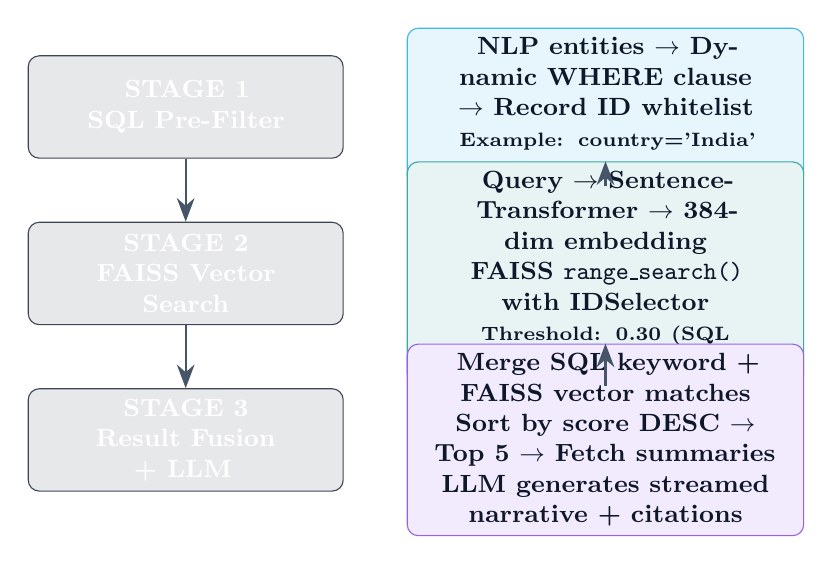
\begin{tikzpicture}[node distance=0.4cm and 0.6cm, every node/.style={font=\small}]

  % Stage 1
  \node[component=navy, minimum width=4cm, text=white, minimum height=1.3cm] (s1title) {\textbf{STAGE 1}\\SQL Pre-Filter};
  \node[component=skyblue, right=0.8cm of s1title, minimum width=5cm, text width=4.8cm] (s1desc) {NLP entities $\rightarrow$ Dynamic WHERE clause\\$\rightarrow$ Record ID whitelist\\{\scriptsize Example: country='India' AND trouble\_code='P0500'}};

  % Stage 2
  \node[component=navy, below=0.8cm of s1title, minimum width=4cm, text=white, minimum height=1.3cm] (s2title) {\textbf{STAGE 2}\\FAISS Vector Search};
  \node[component=teal, right=0.8cm of s2title, minimum width=5cm, text width=4.8cm] (s2desc) {Query $\rightarrow$ SentenceTransformer $\rightarrow$ 384-dim embedding\\FAISS \texttt{range\_search()} with IDSelector\\{\scriptsize Threshold: 0.30 (SQL match) / 0.45 (no match)}};

  % Stage 3
  \node[component=navy, below=0.8cm of s2title, minimum width=4cm, text=white, minimum height=1.3cm] (s3title) {\textbf{STAGE 3}\\Result Fusion + LLM};
  \node[component=violet, right=0.8cm of s3title, minimum width=5cm, text width=4.8cm] (s3desc) {Merge SQL keyword + FAISS vector matches\\Sort by score DESC $\rightarrow$ Top 5 $\rightarrow$ Fetch summaries\\LLM generates streamed narrative + citations};

  % Arrows
  \draw[flow] (s1title) -- (s2title);
  \draw[flow] (s2title) -- (s3title);
  \draw[flow] (s1desc) -- (s2desc);
  \draw[flow] (s2desc) -- (s3desc);

\end{tikzpicture}
\caption{Three-Stage Hybrid Retrieval Architecture}
\label{fig:retrieval}
\end{figure}

\subsection{Vector Index Architecture}

\begin{table}[H]
\centering
\caption{FAISS Vector Index Specifications}
\label{tab:faiss}
\rowcolors{2}{slate50}{white}
\begin{tabularx}{\textwidth}{L{2.8cm} L{3.5cm} X}
\toprule
\rowcolor{darknavy}\color{white}\textbf{Parameter} & \color{white}\textbf{Value} & \color{white}\textbf{Rationale} \\
\midrule
Index Type & IndexFlatIP + IndexIDMap & Exact inner product search with custom record IDs \\
Embedding Model & all-MiniLM-L6-v2 & 384-dim, fast inference, strong semantic similarity \\
Similarity Metric & Cosine (via normalized IP) & L2 normalized vectors $\Rightarrow$ IP $=$ Cosine \\
Document Fields & 6 concatenated text fields & subject, complaint, checked, results, repair, part \\
Metadata & id, country, model, code, segment & Enables pre-filter ID selection \\
Search Method & \texttt{range\_search()} + \texttt{IDSelectorArray} & Threshold-based filtering on whitelisted subset \\
Persistence & faiss\_index.bin + vector\_metadata.json & Binary index + JSON metadata on disk \\
\bottomrule
\end{tabularx}
\end{table}

\subsection{Embedding Cache Strategy}

To avoid redundant SentenceTransformer inference, all computed embeddings are cached in the \texttt{embedding\_cache} SQLite table as BLOB-serialized NumPy arrays. The cache key is an MD5 hash of the input text, providing $O(1)$ lookup. This is critical during ETL batch ingestion where thousands of documents are processed.

\subsection{SQL Keyword Search (BM25-like)}

Alongside vector search, the system performs keyword-based SQL LIKE queries across four text columns: \texttt{subject}, \texttt{customer\_complaint}, \texttt{causal\_parts\_name}, and \texttt{summary}. Keywords are extracted by the NLP pipeline (nouns, proper nouns, adjectives) with stop-word filtering. Results are intersected with metadata-whitelisted IDs and merged with FAISS scores (baseline score = 0.35 for SQL-only matches).

\newpage

% ══════════════════════════════════════════════════════════════════════════════
%  SECTION 10: FRONTEND ARCHITECTURE
% ══════════════════════════════════════════════════════════════════════════════
\section{Frontend Architecture}

The frontend is built with \textbf{Streamlit} and features a multi-page layout with three main views, custom enterprise CSS theming (Inter font family, glassmorphism cards), and interactive chat with streaming LLM responses.

\subsection{Page Structure}

\begin{table}[H]
\centering
\caption{Frontend Page Structure}
\label{tab:pages}
\rowcolors{2}{slate50}{white}
\begin{tabularx}{\textwidth}{L{2.5cm} L{2.8cm} X}
\toprule
\rowcolor{navy}\color{white}\textbf{Page} & \color{white}\textbf{Route} & \color{white}\textbf{Features} \\
\midrule
AI Chat \& RAG & \faIcon{comments} AI Chat \& RAG & Chat interface, streamed LLM, citation cards, SQL viewer, Plotly charts, PDF export \\
Quality Dashboard & \faIcon{chart-bar} Quality Dashboard & 4 KPI metric cards, trouble code chart, trend line, quality donut, model comparison \\
Monthly Reports & \faIcon{file-pdf} Monthly Reports & Year/month selector, PDF + DOCX generation, download buttons \\
\bottomrule
\end{tabularx}
\end{table}

\subsection{UI Component Hierarchy}

\begin{figure}[H]
\centering
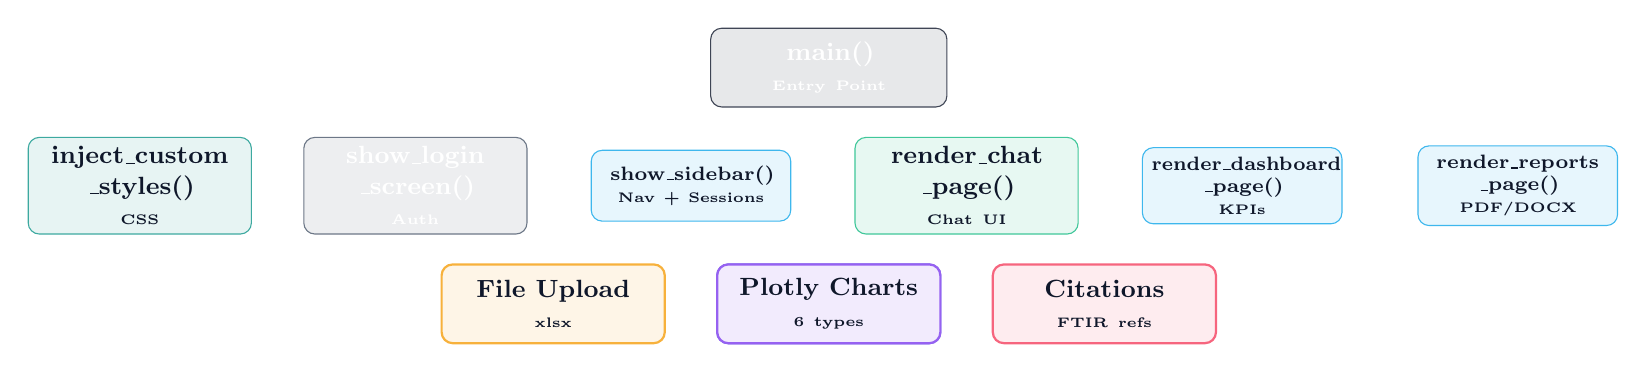
\begin{tikzpicture}[
  grow=down,
  sibling distance=3.5cm,
  level distance=1.5cm,
  edge from parent/.style={flow},
  every node/.style={component=skyblue, minimum width=2.5cm, text width=2.3cm, minimum height=0.9cm, font=\scriptsize\bfseries}
]
  \node[component=navy, text=white, minimum width=3cm] {main()\\{\tiny Entry Point}}
    child { node[component=teal] {inject\_custom\\\_styles()\\{\tiny CSS}} }
    child { node[component=slate600, text=white] {show\_login\\\_screen()\\{\tiny Auth}}
    }
    child { node {show\_sidebar()\\{\tiny Nav + Sessions}}
      child { node[component=amber] {File Upload\\{\tiny xlsx}} }
      child { node[component=indigo] {Chat Sessions\\{\tiny CRUD}} }
    }
    child { node[component=emerald] {render\_chat\\\_page()\\{\tiny Chat UI}}
      child { node[component=violet] {Plotly Charts\\{\tiny 6 types}} }
      child { node[component=rose] {Citations\\{\tiny FTIR refs}} }
    }
    child { node {render\_dashboard\\\_page()\\{\tiny KPIs}} }
    child { node {render\_reports\\\_page()\\{\tiny PDF/DOCX}} };

\end{tikzpicture}
\caption{Frontend Component Hierarchy Tree}
\label{fig:ui-tree}
\end{figure}

\subsection{Visualization Chart Types}

\begin{table}[H]
\centering
\caption{Dynamic Chart Type Selection (GraphSelector)}
\label{tab:charts}
\rowcolors{2}{slate50}{white}
\begin{tabularx}{\textwidth}{L{2.2cm} L{2.8cm} L{2.5cm} X}
\toprule
\rowcolor{darknavy}\color{white}\textbf{Chart Type} & \color{white}\textbf{Function} & \color{white}\textbf{Use Case} & \color{white}\textbf{Auto-Selected When} \\
\midrule
horizontal\_bar & plot\_horizontal\_bar() & Rankings & failures/count column detected \\
line & plot\_line\_trend() & Temporal trends & period/report\_year column \\
donut & plot\_donut\_chart() & Distribution & quality column + 2 cols only \\
histogram & plot\_histogram() & Mileage dist. & mileage column detected \\
radar & plot\_radar\_comparison() & Multi-metric & COMPARE + resolution\_rate \\
grouped\_bar & plot\_grouped\_bar() & Comparison & 3+ numeric columns \\
\bottomrule
\end{tabularx}
\end{table}

\newpage

% ══════════════════════════════════════════════════════════════════════════════
%  SECTION 11: DEPLOYMENT ARCHITECTURE
% ══════════════════════════════════════════════════════════════════════════════
\section{Deployment Architecture}

The system is designed for \textbf{single-node on-premise deployment} on Windows or Linux workstations with NVIDIA GPU acceleration. No cloud services, API keys, or network connectivity are required.

\begin{figure}[H]
\centering
\begin{tikzpicture}[node distance=0.6cm and 0.6cm, every node/.style={font=\small}]

  % Server box
  \node[draw=navy, very thick, rounded corners=8pt, fill=slate50, minimum width=13cm, minimum height=8cm, label={[font=\bfseries\color{navy}]above:\faIcon{server} On-Premise Workstation / Server}] (server) {};

  % Streamlit
  \node[component=skyblue, minimum width=10cm, text width=9.5cm] at ([yshift=2.5cm]server.center) (streamlit) {\faIcon{desktop} Streamlit Application Server\\{\scriptsize streamlit run app/main.py — Port 8501}};

  % Three storage nodes
  \node[component=indigo, minimum width=3cm] at ([yshift=0.2cm, xshift=-3.5cm]server.center) (sqlitenode) {\faIcon{database} SQLite DB\\{\scriptsize WAL mode}\\{\scriptsize $\sim$6.7 MB}};
  \node[component=teal, minimum width=3cm] at ([yshift=0.2cm]server.center) (faissnode) {\faIcon{search} FAISS Index\\{\scriptsize in-memory}\\{\scriptsize $\sim$9.5 MB}};
  \node[component=violet, minimum width=3cm] at ([yshift=0.2cm, xshift=3.5cm]server.center) (modelnode) {\faIcon{microchip} Phi-3 GGUF\\{\scriptsize CUDA VRAM}\\{\scriptsize $\sim$2.4 GB}};

  % GPU
  \node[component=amber, minimum width=10cm, text width=9.5cm] at ([yshift=-2cm]server.center) (gpu) {\faIcon{bolt} NVIDIA CUDA GPU\\{\scriptsize n\_gpu\_layers=-1 (full offload) | use\_mlock=True}};

  % Arrows
  \draw[flow] (streamlit) -- (sqlitenode);
  \draw[flow] (streamlit) -- (faissnode);
  \draw[flow] (streamlit) -- (modelnode);
  \draw[flow] (modelnode) -- (gpu);

\end{tikzpicture}
\caption{Deployment Topology}
\label{fig:deployment}
\end{figure}

\subsection{System Requirements}

\begin{table}[H]
\centering
\caption{Hardware \& Software Requirements}
\label{tab:requirements}
\rowcolors{2}{slate50}{white}
\begin{tabularx}{\textwidth}{L{2.5cm} X X}
\toprule
\rowcolor{navy}\color{white}\textbf{Resource} & \color{white}\textbf{Minimum} & \color{white}\textbf{Recommended} \\
\midrule
RAM & 8 GB & 16+ GB \\
GPU VRAM & 4 GB (NVIDIA CUDA) & 8+ GB \\
Disk Space & 10 GB & 20+ GB (models + data growth) \\
Python & 3.9+ & 3.10+ \\
CUDA Toolkit & 11.x+ & 12.x \\
OS & Windows 10+ / Linux & Windows 11 / Ubuntu 22.04 \\
\bottomrule
\end{tabularx}
\end{table}

\subsection{Startup Commands}

\begin{lstlisting}[language=bash, caption={Application Launch Commands}]
# Initial setup (one-time):
cd automotive_qa
pip install -r requirements.txt
python setup.py

# Launch application:
streamlit run app/main.py
\end{lstlisting}

\newpage

% ══════════════════════════════════════════════════════════════════════════════
%  SECTION 12: SCALABILITY CONSIDERATIONS
% ══════════════════════════════════════════════════════════════════════════════
\section{Scalability Considerations}

\begin{table}[H]
\centering
\caption{Scalability Assessment \& Mitigation Strategies}
\label{tab:scalability}
\rowcolors{2}{slate50}{white}
\begin{tabularx}{\textwidth}{L{1.8cm} L{2.5cm} X L{2cm}}
\toprule
\rowcolor{navy}\color{white}\textbf{Dimension} & \color{white}\textbf{Current Design} & \color{white}\textbf{Scaling Strategy} & \color{white}\textbf{Threshold} \\
\midrule
Record Count & SQLite single-file & Migrate to PostgreSQL with partitioning & $>$ 500K records \\
Vector Index & FAISS IndexFlatIP & Switch to FAISS IVF-PQ or HNSW & $>$ 1M vectors \\
LLM Inference & Single Phi-3 on 1 GPU & Model parallelism, vLLM, or batching & $>$ 10 concurrent \\
Concurrent Users & Streamlit single-threaded & NGINX + multiple Streamlit workers & $>$ 5 concurrent \\
ETL Volume & Row-by-row insertion & Batch INSERT with \texttt{executemany()} & $>$ 10K rows/file \\
Cache Size & 200-entry RAM LRU & Redis with configurable TTL & $>$ 1000 queries/day \\
Embeddings & CPU + GPU inference & Pre-computed embeddings, batch encoding & $>$ 50K documents \\
\bottomrule
\end{tabularx}
\end{table}

\newpage

% ══════════════════════════════════════════════════════════════════════════════
%  SECTION 13: PERFORMANCE OPTIMIZATIONS
% ══════════════════════════════════════════════════════════════════════════════
\section{Performance Optimizations}

The system implements \textbf{10 key performance optimizations} spanning caching, indexing, model management, and query execution.

\begin{table}[H]
\centering
\caption{Performance Optimization Matrix}
\label{tab:perf}
\rowcolors{2}{slate50}{white}
\begin{tabularx}{\textwidth}{L{2.8cm} X L{3.5cm}}
\toprule
\rowcolor{darknavy}\color{white}\textbf{Optimization} & \color{white}\textbf{Implementation} & \color{white}\textbf{Impact} \\
\midrule
Two-Tier Query Cache & L1 RAM (dict, 200 entries) + L2 SQLite (TTL 2 hours) & Eliminates duplicate LLM calls \\
Embedding Cache & SQLite BLOB storage of NumPy arrays (MD5 key) & Avoids re-encoding in ETL \\
Singleton Resources & \texttt{@st.cache\_resource} for DB, LLM, FAISS & One-time model loading \\
WAL Journal Mode & \texttt{PRAGMA journal\_mode=WAL} & Concurrent reads during writes \\
FAISS IDSelector & Pre-filter search with \texttt{IDSelectorArray} & Reduces vector comparisons \\
Dynamic Threshold & 0.30 (SQL match) vs 0.45 (no match) & Reduces false positives \\
Table Truncation & \texttt{df.head(20)} + \texttt{describe()} for large DFs & Prevents context overflow \\
9 B-Tree Indexes & 95\% filter pattern coverage & Sub-ms SQL execution \\
GPU Full Offload & \texttt{n\_gpu\_layers=-1} + \texttt{use\_mlock=True} & Max LLM throughput \\
Materialized Views & 5 pre-aggregated tables & $O(1)$ dashboard queries \\
\bottomrule
\end{tabularx}
\end{table}

\begin{infobox}[\faIcon{tachometer-alt} Caching Architecture Detail]
The two-tier cache operates as follows:

\begin{enumerate}[itemsep=2pt]
  \item \textbf{L1 (RAM):} An in-memory Python dictionary keyed by MD5 hash of the query string. Maximum 200 entries with automatic FIFO eviction and expiration-based pruning.
  \item \textbf{L2 (SQLite):} Persistent \texttt{query\_cache} table storing JSON-serialized results with configurable TTL (default 2 hours). Supports both user-scoped and globally shared cache entries.
\end{enumerate}

On cache \textit{hit}, the full router response (including DataFrames, chart types, and citations) is returned instantly without invoking the LLM or FAISS subsystems.
\end{infobox}

\newpage

% ══════════════════════════════════════════════════════════════════════════════
%  SECTION 14: SECURITY CONSIDERATIONS
% ══════════════════════════════════════════════════════════════════════════════
\section{Security Considerations}

\begin{table}[H]
\centering
\caption{Security Assessment Matrix}
\label{tab:security}
\rowcolors{2}{slate50}{white}
\begin{tabularx}{\textwidth}{L{2.2cm} X L{3cm}}
\toprule
\rowcolor{navy}\color{white}\textbf{Domain} & \color{white}\textbf{Implementation} & \color{white}\textbf{Assessment} \\
\midrule
Authentication & Passwordless username-based login (\texttt{verify\_or\_create\_user}) & Trusted internal only \\
Data Isolation & User-scoped chat sessions (user\_id FK) & Own history only \\
Data at Rest & SQLite with OS-level file permissions & No encryption \\
Data in Transit & Localhost only (no network exposure) & No TLS needed \\
AI Privacy & Fully offline LLM — no external API calls & No data egress risk \\
SQL Injection & Parameterized queries (\texttt{?}) throughout & Fully protected \\
File Upload & Restricted to \texttt{.xlsx} only via Streamlit uploader & Type validation \\
LLM Safety & Temperature 0.1 + strict stop tokens & Minimal hallucination \\
Sessions & Streamlit \texttt{session\_state} (per browser tab) & Cleared on logout \\
\bottomrule
\end{tabularx}
\end{table}

\begin{warnbox}[\faIcon{exclamation-triangle} Security Advisory]
The current authentication is \textbf{passwordless} and suitable only for trusted internal networks. For production deployment exposed to wider networks, implement:
\begin{itemize}[itemsep=2pt]
  \item Password hashing via \texttt{bcrypt}
  \item JWT-based session tokens
  \item Role-based access control (RBAC): admin, analyst, viewer
  \item HTTPS termination via reverse proxy (NGINX + TLS certificates)
\end{itemize}
\end{warnbox}

\newpage

% ══════════════════════════════════════════════════════════════════════════════
%  SECTION 15: ERROR HANDLING & RESILIENCE
% ══════════════════════════════════════════════════════════════════════════════
\section{Error Handling \& Resilience}

The system implements comprehensive error handling with \textbf{graceful degradation} at every layer:

\begin{table}[H]
\centering
\caption{Error Handling Strategy Matrix}
\label{tab:errors}
\rowcolors{2}{slate50}{white}
\begin{tabularx}{\textwidth}{L{3cm} X L{2.5cm}}
\toprule
\rowcolor{navy}\color{white}\textbf{Error Scenario} & \color{white}\textbf{Handling Strategy} & \color{white}\textbf{Module} \\
\midrule
LLM SQL generation failure & 4-retry self-healing with error context injection & analytics/engine \\
LLM model file not found & \texttt{FileNotFoundError} with descriptive message & llm/client \\
spaCy model not installed & Fallback to regex-only NER extraction & nlp/pipeline \\
FAISS index missing & Automatic rebuild from database records & rag/embedder \\
Duplicate FTIR records & MD5 hash + UNIQUE constraint $\rightarrow$ skip silently & etl/pipeline \\
Excel column name mismatch & Column rename normalization map & etl/pipeline \\
Date parsing failure & Try 4 formats; fallback to raw string & etl/pipeline \\
LLM summary failure & Heuristic 2-sentence summary fallback & etl/pipeline \\
Unrelated user query & FAISS threshold filter $\rightarrow$ general assistant fallback & core/router \\
Empty analytics result & \texttt{text\_stream}: ``No data available'' & core/router \\
Chat session deletion & CASCADE delete of chat\_history records & auth/session \\
Query cache expiry & Auto-delete from SQLite on next access & core/cache \\
MV refresh failure & ROLLBACK transaction; log error & analytics/views \\
CUDA DLL not found & Dynamic DLL directory registration at startup & core/singletons \\
\bottomrule
\end{tabularx}
\end{table}

\newpage

% ══════════════════════════════════════════════════════════════════════════════
%  SECTION 16: FUTURE IMPROVEMENTS
% ══════════════════════════════════════════════════════════════════════════════
\section{Future Improvements}

\subsection{Short-Term Enhancements}

\begin{itemize}[leftmargin=*, itemsep=4pt]
  \item \textbf{Multi-Turn Conversation Context:} Pass previous chat messages to the LLM for context-aware follow-up answers.
  \item \textbf{Advanced Authentication:} Add password hashing (bcrypt), role-based access control, and JWT session tokens.
  \item \textbf{Chart Embedding in Reports:} Render Plotly charts as PNG images and embed them in monthly PDF reports.
  \item \textbf{Real-Time ETL Watchdog:} Use filesystem event monitoring (\texttt{watchdog} library) for automatic inbox ingestion.
  \item \textbf{Batch ETL Optimization:} Replace row-by-row INSERT with \texttt{executemany()} for 10$\times$+ ingestion performance.
\end{itemize}

\subsection{Medium-Term Enhancements}

\begin{itemize}[leftmargin=*, itemsep=4pt]
  \item \textbf{PostgreSQL Migration:} Replace SQLite with PostgreSQL for true concurrent multi-user access and table partitioning.
  \item \textbf{FAISS IVF-PQ Index:} Upgrade to Inverted File with Product Quantization for sub-linear search at 1M+ scale.
  \item \textbf{Larger LLM Models:} Support Qwen 2.5 7B (already downloaded) or Llama 3.1 for improved SQL generation.
  \item \textbf{REST API Layer:} Expose FastAPI endpoints for headless integration with other enterprise systems.
  \item \textbf{Automated Testing:} Add \texttt{pytest} suite covering NLP classification, ETL pipeline, and analytics correctness.
\end{itemize}

\subsection{Long-Term Vision}

\begin{itemize}[leftmargin=*, itemsep=4pt]
  \item \textbf{Kubernetes Deployment:} Containerize (Docker) and deploy on K8s with horizontal pod autoscaling.
  \item \textbf{Real-Time Streaming:} Integrate with Kafka or MQTT for live field data from IoT-connected vehicles.
  \item \textbf{Predictive Analytics:} Train time-series models (Prophet/ARIMA) on failure trends for proactive alerts.
  \item \textbf{Knowledge Graph:} Build a Neo4j knowledge graph linking models, parts, failure modes, and repairs.
  \item \textbf{Multi-Language Support:} Extend NLP pipeline for Japanese, Korean, and other OEM-relevant languages.
\end{itemize}

\newpage

% ══════════════════════════════════════════════════════════════════════════════
%  SECTION 17: TECHNOLOGY STACK SUMMARY
% ══════════════════════════════════════════════════════════════════════════════
\section{Technology Stack Summary}

\begin{table}[H]
\centering
\caption{Complete Technology Stack}
\label{tab:tech-stack}
\rowcolors{2}{slate50}{white}
\begin{tabularx}{\textwidth}{L{2cm} L{2.8cm} L{3cm} X}
\toprule
\rowcolor{navy}\color{white}\textbf{Category} & \color{white}\textbf{Technology} & \color{white}\textbf{Version} & \color{white}\textbf{Role} \\
\midrule
Language & Python & 3.9+ & Primary development language \\
Web Framework & Streamlit & 1.x & Frontend UI and application server \\
Database & SQLite 3 & WAL mode & Structured data storage \\
Vector Store & FAISS (faiss-cpu) & 1.x & 384-dim cosine similarity index \\
Embedding & SentenceTransformers & all-MiniLM-L6-v2 & Text $\rightarrow$ 384-dim vector encoding \\
LLM Runtime & llama-cpp-python & CUDA build & Local GGUF model inference \\
LLM Model & Phi-3 Mini 4K & Q4 GGUF (2.4 GB) & Chat, summary, SQL generation \\
NLP & spaCy & en\_core\_web\_sm & NER and keyword extraction \\
Visualization & Plotly & Express + GO & 6 interactive chart types \\
Data Processing & Pandas & 2.x & DataFrame operations \\
PDF Generation & ReportLab & 4.x & Professional PDF rendering \\
DOCX Generation & python-docx & 0.8+ & Word document reports \\
Excel Parsing & openpyxl & 3.x & FTIR Excel file reading \\
Numerical & NumPy & 1.x & Vector array operations \\
GPU Acceleration & NVIDIA CUDA & 11.x+ & LLM inference GPU offloading \\
\bottomrule
\end{tabularx}
\end{table}

\vspace{1cm}

\begin{center}
  {\color{skyblue}\rule{6cm}{1.5pt}}\\[0.5cm]
  {\color{slate400}\large — End of Document —}\\[0.3cm]
  {\color{slate500}\small Document generated on \today}\\[0.2cm]
  {\color{slate500}\footnotesize Automotive QA Intelligence — System Architecture Documentation v1.1}
\end{center}

\end{document}
